\chapter{Исследовательская часть}

В данном разделе будут приведены исследование временных характеристик реализуемых алгоритмов и оценка их затрат по памяти.

\section{Технические характеристики}

Технические характеристики устройства, на котором выполнялись замеры по времени:

\begin{itemize}
    \item Процессор: Intel i5-1035G1 (8) @ 3.600 ГГц.
    \item Оперативная память: 16 ГБайт.
    \item Операционная система: Manjaro Linux x86\_64 (версия ядра Linux 5.15.131-1-MANJARO).
\end{itemize}

Во время проведения измерений времени ноутбук был подключен к сети электропитания и был нагружен только системными приложениями.

\section{Демонстрация работы программы}

На рисунке \ref{fig:prog-demo} демонстрация работы программы для случая, когда пользователь выбирает опцию 1 <<Сортировка массива>> и передает в программу массив $[5, 3, 2, 9, 7]$.

\begin{figure}[H]
    \centering
    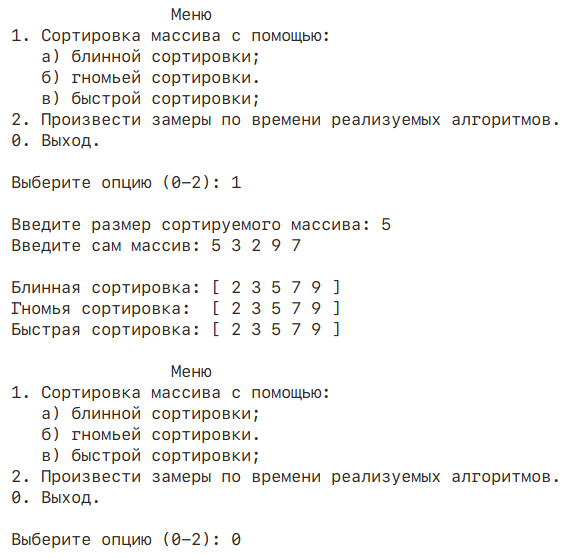
\includegraphics[width=0.8\textwidth]{images/prog_demo.png}
    \caption{Демонстрация работы программы}
    \label{fig:prog-demo}
\end{figure}

\section{Временные характеристики}

\section{Характеристики по памяти}

\section{Вывод}
\addcontentsline{toc}{section}{Вывод}
